\let\negmedspace\undefined
\let\negthickspace\undefined
\documentclass[journal]{IEEEtran}
\usepackage[a5paper, margin=10mm, onecolumn]{geometry}
\usepackage{lmodern} % Ensure lmodern is loaded for pdflatex
\usepackage{tfrupee} % Include tfrupee package

\setlength{\headheight}{1cm} % Set the height of the header box
\setlength{\headsep}{0mm}     % Set the distance between the header box and the top of the text

\usepackage{gvv-book}
\usepackage{gvv}
\usepackage{cite}
\usepackage{amsmath,amssymb,amsfonts,amsthm}
\usepackage{algorithmic}
\usepackage{graphicx}
\usepackage{textcomp}
\usepackage{xcolor}
\usepackage{txfonts}
\usepackage{listings}
\usepackage{enumitem}
\usepackage{mathtools}
\usepackage{gensymb}
\usepackage{comment}
\usepackage[breaklinks=true]{hyperref}
\usepackage{tkz-euclide} 
\usepackage{listings}                                      
\def\inputGnumericTable{}                                 
\usepackage[latin1]{inputenc}                                
\usepackage{color}                                            
\usepackage{array}                                            
\usepackage{longtable}
\usepackage{multicol}
\usepackage{calc}                                             
\usepackage{multirow}                                         
\usepackage{hhline}                                           
\usepackage{ifthen}                                           
\usepackage{lscape}
\begin{document}

\bibliographystyle{IEEEtran}
\vspace{3cm}

\title{9.1.7}
\author{EE24BTECH11006 - Arnav Mahishi}
% \maketitle
% \newpage
% \bigskip
{\let\newpage\relax\maketitle}

\renewcommand{\thefigure}{\theenumi}
\renewcommand{\thetable}{\theenumi}
\setlength{\intextsep}{10pt} % Space between text and floats


\numberwithin{equation}{enumi}
\numberwithin{figure}{enumi}
\renewcommand{\thetable}{\theenumi}


\textbf{Question}:\newline
Solve the differential equation $y^{\prime\prime\prime}+2y^{\prime\prime}+y^{\prime} = 0$ with initial conditions $y\brak{0} = 1$,$y^{\prime}\brak{0} = -1$ , and $y^{\prime\prime}\brak{0} = 1$
\newline
\textbf{Solution: }
\begin{table}[h!]    
  \centering
  \begin{tabular}[10pt]{ |c| c| c|}
    \hline
    \textbf{input}&\textbf{Description}&\textbf{value}\\
    \hline 
    $a$&Length of semi major axis of ellipse&$3$\\
    \hline
    $b$&Length of semi minor axis of ellipse&$2$\\
    \hline
    $v$&Quadratic form of matrix&$\myvec{b^2&0\\0&a^2}$\\
    \hline 
    $u$&Linear coefficient vector&$0$\\
    \hline 
    $f$&Constant Term&$-(a^2b^2)$\\
    \hline
    $h$&One of the points the line passes through&$\myvec{a\\0}$\\
    \hline
    $m$&Slope of line&$\myvec{\frac{1}{b}\\\frac{-1}{a}}$\\
    \hline
    $n$& number of subintervals we are taking & $1000$\\
    \hline
    $x_0$&$x$ coordinate of first intersection point& $3$\\
    \hline
    $x_n$& $y$ coordinate of second intersection point& $2$\\
    \hline
    \end{tabular}

  \caption{Variables Used}
  \label{tab1.1.2.2}
\end{table}
\newline
Theoretical Solution:
We apply the Laplace transform to each term in the equation. The Laplace transforms for the derivatives of $y\brak{t}$ are:
\begin{align}
\mathcal{L}\fbrak{y^{\prime}\brak{t}} &= sY\brak{s} - y\brak{0}\\
\mathcal{L}\{y^{\prime\prime}\brak{t}\} &= s^2Y\brak{s} - s y\brak{0} - y^{\prime}\brak{0}\\
\mathcal{L}\{y^{\prime\prime\prime}\brak{t}\} &= s^3Y\brak{s} - s^2 y\brak{0} - sy^{\prime}\brak{0} - y^{\prime\prime}\brak{0}
\end{align}
Now, applying the Laplace transform to the entire differential equation:
\begin{align}
\mathcal{L}\{y^{\prime\prime\prime} + 2y^{\prime\prime} + y^{\prime}\} = 0\\
\mathcal{L}\{y^{\prime\prime\prime}\brak{t}\} + 2\mathcal{L}\{y^{\prime\prime}\brak{t}\} + \mathcal{L}\{y^{\prime}\brak{t}\} = 0 \\
(s^3 Y\brak{s} - s^2 y\brak{0} - s y^{\prime}\brak{0} - y^{\prime\prime}\brak{0}) + 2(s^2 Y\brak{s} - s y\brak{0} - y^{\prime}\brak{0}) + (s Y\brak{s} - y\brak{0}) = 0
\end{align}
Substitute the initial conditions $y\brak{0} = 1$, $y^{\prime}\brak{0} = -1$, and $y^{\prime\prime}\brak{0} = 1$:
\begin{align}
\brak{s^3 Y\brak{s} - s^2 \cdot 1 - s \cdot (-1) - 1} + 2\brak{s^2 Y\brak{s} - s \cdot 1 - (-1)} + \brak{s Y\brak{s} - 1} &= 0 \\
s^3 Y\brak{s} - s^2 + s - 1 + 2s^2 Y\brak{s} - 2s + 2 + s Y\brak{s} - 1 &= 0
\end{align}

Simplify the equation:

\begin{align}
&(s^3 + 2s^2 + s) Y\brak{s} - (s^2 - s + 1) - (2s - 2) - 1 &= 0 \\
&(s^3 + 2s^2 + s) Y\brak{s} - s^2 - s + 1 - 2s + 2 - 1 &= 0 \\
&(s^3 + 2s^2 + s) Y\brak{s} - (s^2 + s) &= 0
\end{align}
Now, solve for \( Y\brak{s} \):
\begin{align}
\brak{s^3 + 2s^2 + s} Y\brak{s} &= s^2 + s \\
Y\brak{s} &= \frac{s^2 + s}{s(s+1)^2}\\
\implies Y\brak{s} &= \frac{1}{s + 1}
\end{align}
Now, take the inverse Laplace transform:
\begin{align}
\mathcal{L}^{-1}\brak{\frac{1}{s + 1}} = e^{-t}
\end{align}
Thus, the solution to the differential equation is:
\begin{align}
   y\brak{t} = e^{-t} 
\end{align}
\newline
Computational Solution:\\
Consider the given linear differential equation
\begin{align}
	a_{n}y_{n} + a_{n-1}y_{n-1} + \dots + a_{1}y_1 + a_{0}y_{0} + c = 0
\end{align}
Where $y_{i}$ is the $i$th derivative of the function then
\begin{align}
    \myvec{y_{0}^{\prime}\\y_{1}^{\prime}\\y_{2}^{\prime}\\ \vdots\\y^{\prime}_{n-1}}&=\myvec{y_{1}\\y_{2}\\y_{3}\\ \vdots\\ \frac{-\brak{\sum_{i=0}^{i=n-1}a_iy_i}-c}{a_n}}\\
    \implies  \myvec{1\\y_{0}^{\prime}\\y_{1}^{\prime}\\y_{2}^{\prime}\\ \vdots\\y^{\prime}_{n-1}}&=\myvec{1&0&0&\cdots&\cdots&\cdots&\cdots\\0&0&1&0&\cdots&\cdots&\cdots\\0&0&0&1&0&\cdots&\cdots\\0&0&0&0&1&0&\cdots\\ \vdots&\vdots&\vdots&\vdots&\vdots&\vdots&\ddots\\ \frac{-c}{a_n}&\frac{-a_{0}}{a_n}&\frac{-a_{1}}{a_n}&\frac{-a_{2}}{a_n}&\cdots&\cdots&\frac{-a_{n-1}}{a_n}}\myvec{1\\y_{0}\\y_{1}\\y_{2}\\ \vdots\\y_{n-1}}\\
    \implies \overrightarrow{V}^{\prime}\brak{t}&=A\overrightarrow{V}\brak{t}
\end{align}
Where $\overrightarrow{V}\brak{t}$ is the vector $\myvec{1\\y_{0}\\y_{1}\\y_{2}\\ \vdots\\y_{n-1}}$ at a $t$. Using the definition of a derivative we get
\begin{align}
	y^{\prime}\brak{t} &= \lim_{h\to 0}\frac{y\brak{t+h} - y\brak{t}}{h}\\
	y\brak{t+h} &= y\brak{t} + hy^{\prime}\brak{t}\\
    \implies \overrightarrow{V}\brak{t+h}&=\overrightarrow{V}\brak{t}+h\brak{A\overrightarrow{V}\brak{t}}
\end{align}
When $t$ ranges from $t_o$ to $t_f$ in increments of $h$, discretizing the steps gives us all $\overrightarrow{V}\brak{x}$ from $t_o$ to $t_f$ in increments of $h$
Record the $y_0$ for each $\overrightarrow{V}\brak{x}$ we got and then plot the graph. The result will be as given below.
\begin{figure}[h!]
   \centering
   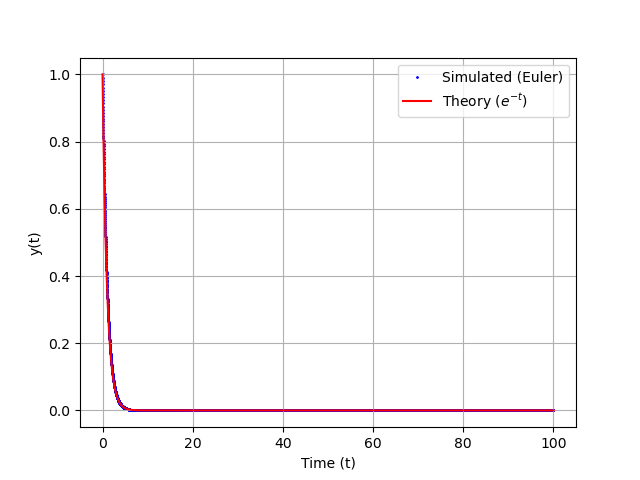
\includegraphics[width=1\linewidth]{figs/fig.png}
   \caption{Comparison between the Theoretical solution and Computational solution}
   \label{stemplot}
\end{figure}
\end{document}

